\newpage
\genHeader

\section{Creating instances}
\hypertarget{sec:creatingInstance common}{}

Before diving into modelling dynamic behaviour in Part III, let's have a brief look at how to create a concrete \emph{instance} of your abstract syntax in
Eclipse.

\vspace{0.5cm}

In the following section, we use \emph{metamodel} and \emph{instance model} to differentiate between models that represent the abstract syntax and static
semantics of a domain specific language (metamodel), and those that are expressed \emph{in} such a language (instance models of the metamodel).

\begin{itemize}

\item[$\blacktriangleright$] To create an instance model, navigate to the generated \texttt{model} folder in your \texttt{LearningBoxLanguage} project.
Double-click the \texttt{LearningBoxLa\-nguage.ecore} model to invoke  the \emph{Ecore model editor}. The Eclipse Modeling Framework (EMF) provides a generic
tree-model editor which allows us to create and edit an arbitrary instance of any metamodel specified with eMoflon. Expand this tree to review all the classes,
attributes, and signatures you just created.

\vspace{0.5cm}

\item[$\blacktriangleright$] To create a concrete instance of the metamodel, you must select a class that will become the root element of the new instance.
For our example, right-click \texttt{Box}, and navigate to ``Create Dynamic Instance'' from the context menu, as depicted in Fig.~\ref{fig:context_menu}.

\begin{figure}[htbp]
	\centering
  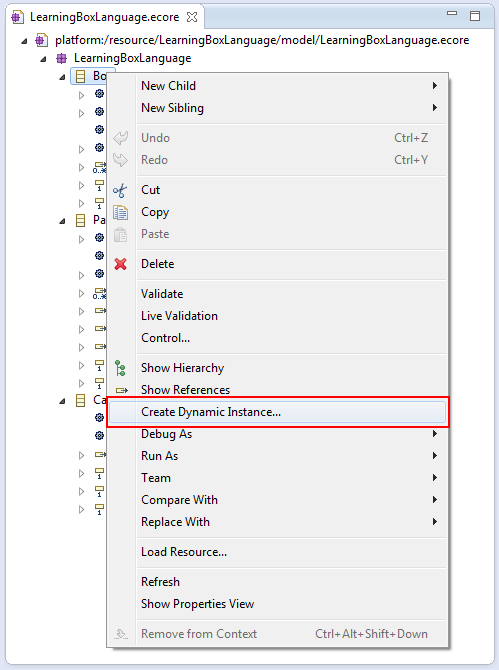
\includegraphics[width=0.6\textwidth]{eclipse_createDynamicInstance}
	\caption{Context menu of an EClass in the Ecore editor}
	\label{fig:context_menu}
\end{figure}

\vspace{0.5cm}

\item[$\blacktriangleright$] A dialogue should appear asking where the instance model file should be persisted. Save your instances according to convention in a
folder named ``instances,'' which is automatically created in every new repository project. Last but not least, enter `Box' as the name of the instance model
(Fig.~\ref{fig:store_dynamic_instance}).

\vspace{0.5cm}

\begin{figure}[htbp]
	\centering
  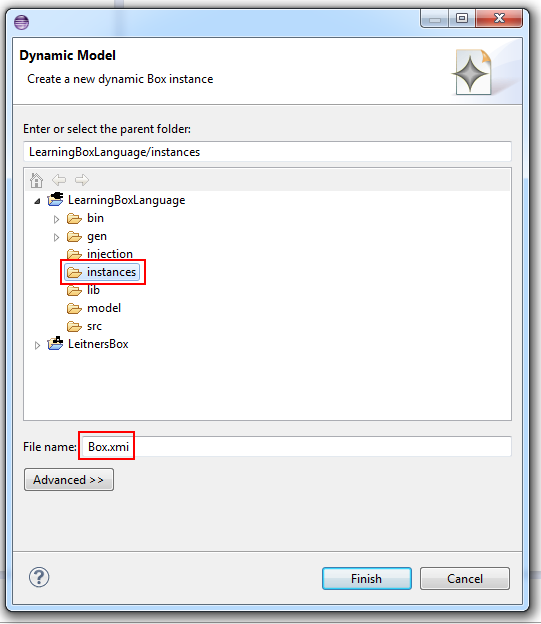
\includegraphics[width=0.6\textwidth]{eclipse_nameDynamicInstance}
	\caption{Dialogue for creating a dynamic model instance}
	\label{fig:store_dynamic_instance}
\end{figure}

\item[$\blacktriangleright$] Press \texttt{Finish}, and the generic model editor should open for your new instance model. This editor works just like the
previous Ecore model editor except it's ``generic,'' meaning it allows you to create and edit an instance of \emph{any} metamodel, not only those using Ecore.

\clearpage

\item[$\blacktriangleright$] You can populate any element of your instance by adding new children or siblings via a right-click of an element to invoke the
context-menu depicted in Fig.~\ref{fig:create_instance}. Note that EMF supports you by respecting your metamodel, and reducing the choice of available elements
to valid types only.\footnote{This depends on the current context. Try it out!}

\begin{figure}[htbp]
	\centering
  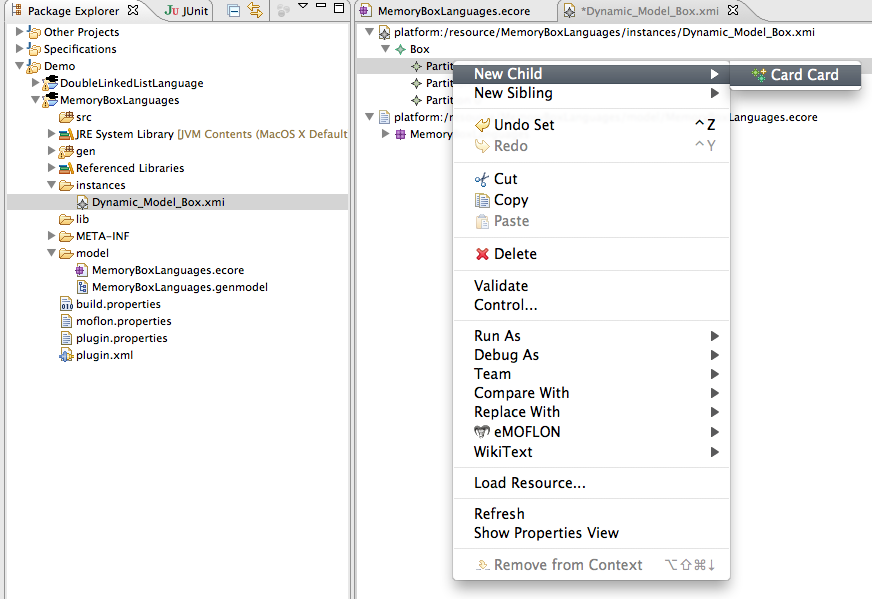
\includegraphics[width=0.8\textwidth]{adjustModel}
	\caption{Context menu for creating model elements}
	\label{fig:create_instance}
\end{figure}

\item[$\blacktriangleright$] Your model as an \texttt{.xmi} file by pressing \texttt{Ctrl+S}. When you close it, the model can be reloaded via a simple
double-click to invoke the generic model editor.

\item[$\blacktriangleright$] Let's try building a vocabulary set. Fill your box with two partitions, each containing three cards.

\item[$\blacktriangleright$] Double click on one of the partitions to bring up the ``Properties'' tab in the window below the editor
(Fig.~\ref{fig:properties_partition}). Here you'll see the attributes you defined earlier in the classes. Pick a number - any one you like - and update the
\texttt{Partition} value. As soon as you hit \texttt{Enter}, you'll see that the change in name has been reflected in the tree. Give the second partition a
unique EInt value as well.

\item[$\blacktriangleright$] Now you need to set the \texttt{Next} and \texttt{Previous} partition values that will make it possible to move cards through the
box. Set every \texttt{Previous} value to the very first partition in your box, then each \texttt{Next} value to the next partition. For the last partition, set
the \texttt{Next} value to itself. 

\item[$\blacktriangleright$] In the same fashion, double click on each \texttt{Card} you created and modify their values. In particular, modify the
\texttt{Back} attribute. Change it to `Null' This is the value you'll see from the partition. You'll be experimenting with the \texttt{Face} attribute shortly,
so provide a `Zero' value for that as well.

\item[$\blacktriangleright$] Fill in the rest the cards with similar vocabulary-style words that you can quiz yourself on. You now have a unique, customized
learning box! Save your model, and ensure no errors exist before proceeding with the final sections of this handbook.

\newpage

\vspace*{4cm}

\begin{figure}[htbp]
	\centering
  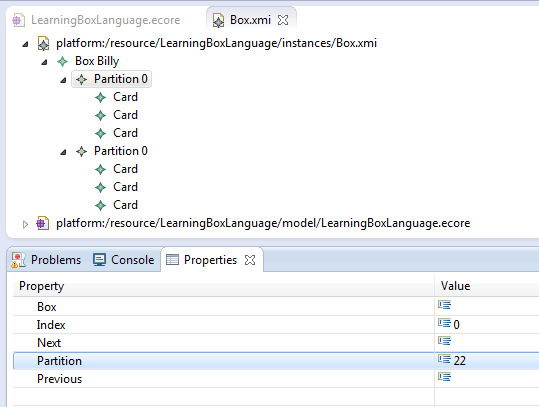
\includegraphics[width=0.8\textwidth]{eclipse_propertiesTab}
	\caption{Change the \texttt{Index} value in the partition's property tab}
	\label{fig:properties_partition}
\end{figure}

% \fancyfoot[R]{ $\triangleright$ \hyperlink{sec:Graph View}{Next}}

\end{itemize}
